\chapter{FastIC+}
\label{sec:fastic}
The FastIC+ is a configurable ASIC for fast timing applications, featuring 8-channel front-end for photo detectors such as SiPM, PMT or MCP, capable of precisely measuring the Time-of-Arrival (ToA) and Time-over-Treshold (ToT) of photons hitting the detectors. This feature set finds it's use in applications that require precise photon timestamping, such as Time-of-Flight Positron Emission Tomography, high-energy physics, mass-spectrometry or LIDAR applications. The ASIC is developed in the \SI{65}{\nano\meter} technology by the Institut de Ciencies del Cosmos of the University of Barcelona in close colaboration with CERN. 

The ASIC can be mostly used without any additional circuitry. Only power and a \SI{40}{\mega\hertz} low jitter reference clock needs to be provided for correct operation. The chip is configured over a I2C interface.

\FloatBarrier
\begin{figure}[htp!]
    \centering
    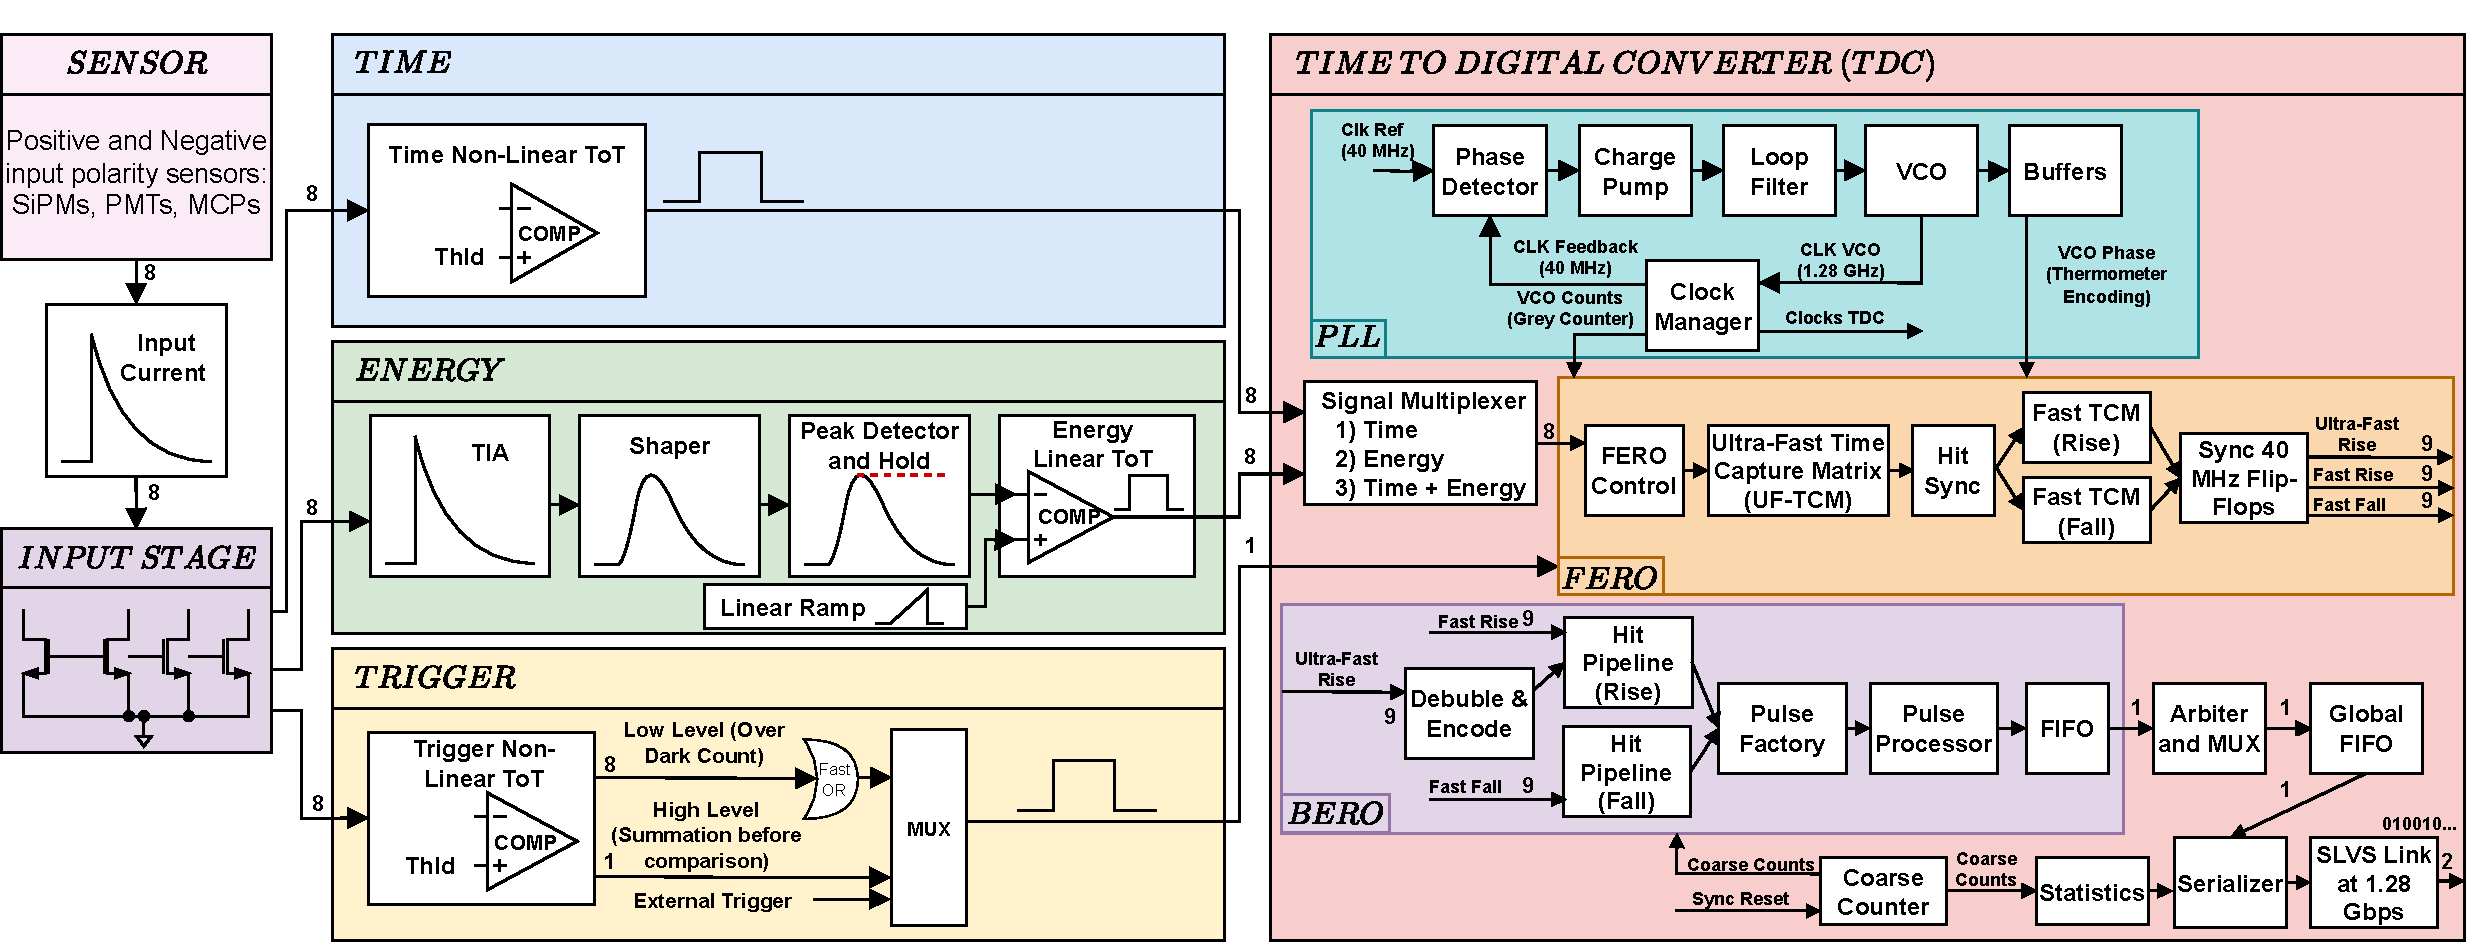
\includegraphics[height=4.8cm]{05_FASTICPLUS_BLOCK.pdf}
    \caption{Top-level architecture block diagram}
    \label{fig:fastic_top_level}
\end{figure}
\FloatBarrier



\section{Detection}
Each channel of the ASIC consists of a low impedance input stage, working with both positive and negative polarity sensors with dynamic range of \SI{5}{\micro\ampere} to \SI{20}{\milli\ampere} and stability across sensor capacitances from \SI{10}{\pico\farad} to \SI{1}{\nano\farad}. This stage generates three differently scaled replicas of the input current pulse and forwards them to the three signal paths: time, energy and trigger.
%
\subsection{Time path}
The time path acts as a simple discriminator which compares the pulse to a programmable treshold, which can be set down to a single photoelectron level. The leading edge of the comparator output pulse provides the ToA timestamp. The logical OR of all time channels can be output via the \verb|TIME| output. 
%
\subsection{Energy path}
The energy path extracts the pulse peak in order to estimate the energy deposited in the sensor. The chain consists of a transimpedance amplifier, shaper, peak detector with hold and a comparator that compares the peak detector level with a linear ramp. The length of the output pulse than directly encodes the energy of the pulse. The input can also be compared to a constant treshold to provide a non-linear ToT instead. 

\subsection{Trigger path}
The final path, the trigger, generates either a low-level trigger per every channel or a cluster trigger. The low-level trigger is an logical OR of all the trigger comparators for all channels whereas the cluster trigger results from a analog summation of the input pulses passed through a single comparator. This trigger can be used internally to trigger the conversion FSM or output on a pin. An external trigger can be provided on a pin aswell.

%Three different measurement modes, 
%\begin{itemize}
%    \item ToA (non-linear ToT),
%    \item Energy (from ToT),
%    \item Hybrid (ToA + Energy),
%\end{itemize}
%are present to allow the user to optimize for measurement of ToA, ToT or both. The maximum detection rate of the impacts is approximately \SI{2}{\mega\hertz} in the linear mode and \SI{50}{\mega\hertz} in non-linear mode.


\section{Digitizing}
\label{sec:fastic_digitizing}
The time, energy, and trigger pulses from each channel are then passed to a Front-End Readout block (FERO), which interpolates the input pulse and obtains a digital representation of the rising edge (with a \SI{25}{\pico\second} time bin) and the falling edge (with a \SI{390}{\pico\second} time bin).

After the edge capture, the timing information is passed to the Back-End Readout Block (BERO), which processes the information. It corrects any signal errors, performs trigger validation and filtering, and encodes the timing information into a suitable binary format. In the end, it stores the encoded packet in the channel's FIFO buffer. An arbiter with a multiplexer (MUX) then handles the requests from all the channel FIFOs and stores the packets in a global FIFO.

As the last step, an Aurora serializer converts the packets from the FIFO into an Aurora 64B/66B serial stream and sends it over the high-speed differential output lines. Statistical and counter information is also sent if enabled. The stream can be configured to run at speeds from \SI{80}{\mega\bit\per\second} to \SI{1.28}{\giga\bit\per\second} in accordance with the Aurora specification.

%\section{Configuration and testing}
%An I2C interface has been implemented alongside the Aurora bus to allow for easy configuration of the chip parameters. This interface can run at speeds up to \SI{1}{\mega\hertz} and can be shared between multiple FastIC+ chips. 

%For testing purposes, four debug pins are exposed to read out the state of the internal FSM. If not used for debugging, they can be utilized for configuration of the I2C address. 
